%---------------------------------------------------------------------------------
% QUESTION 4.A
%---------------------------------------------------------------------------------
\secMOGS{Adding Aerodynamics}

Modify \verb!aero_effects.m! to implement the added downforce and drag from the wing.  We can assume that the front wing aero forces act at the center of the front wheel and that the rear wing aero forces act at a distance \verb!veh.hRwing! directly above the rear wheel. We can also assume that the front wing acts equally on the left and right front wheels and that the rear wing acts equally on the left and right rear wheels. Here is a free body diagram of the GTI with the forces we added with the two wings.    

\begin{center}
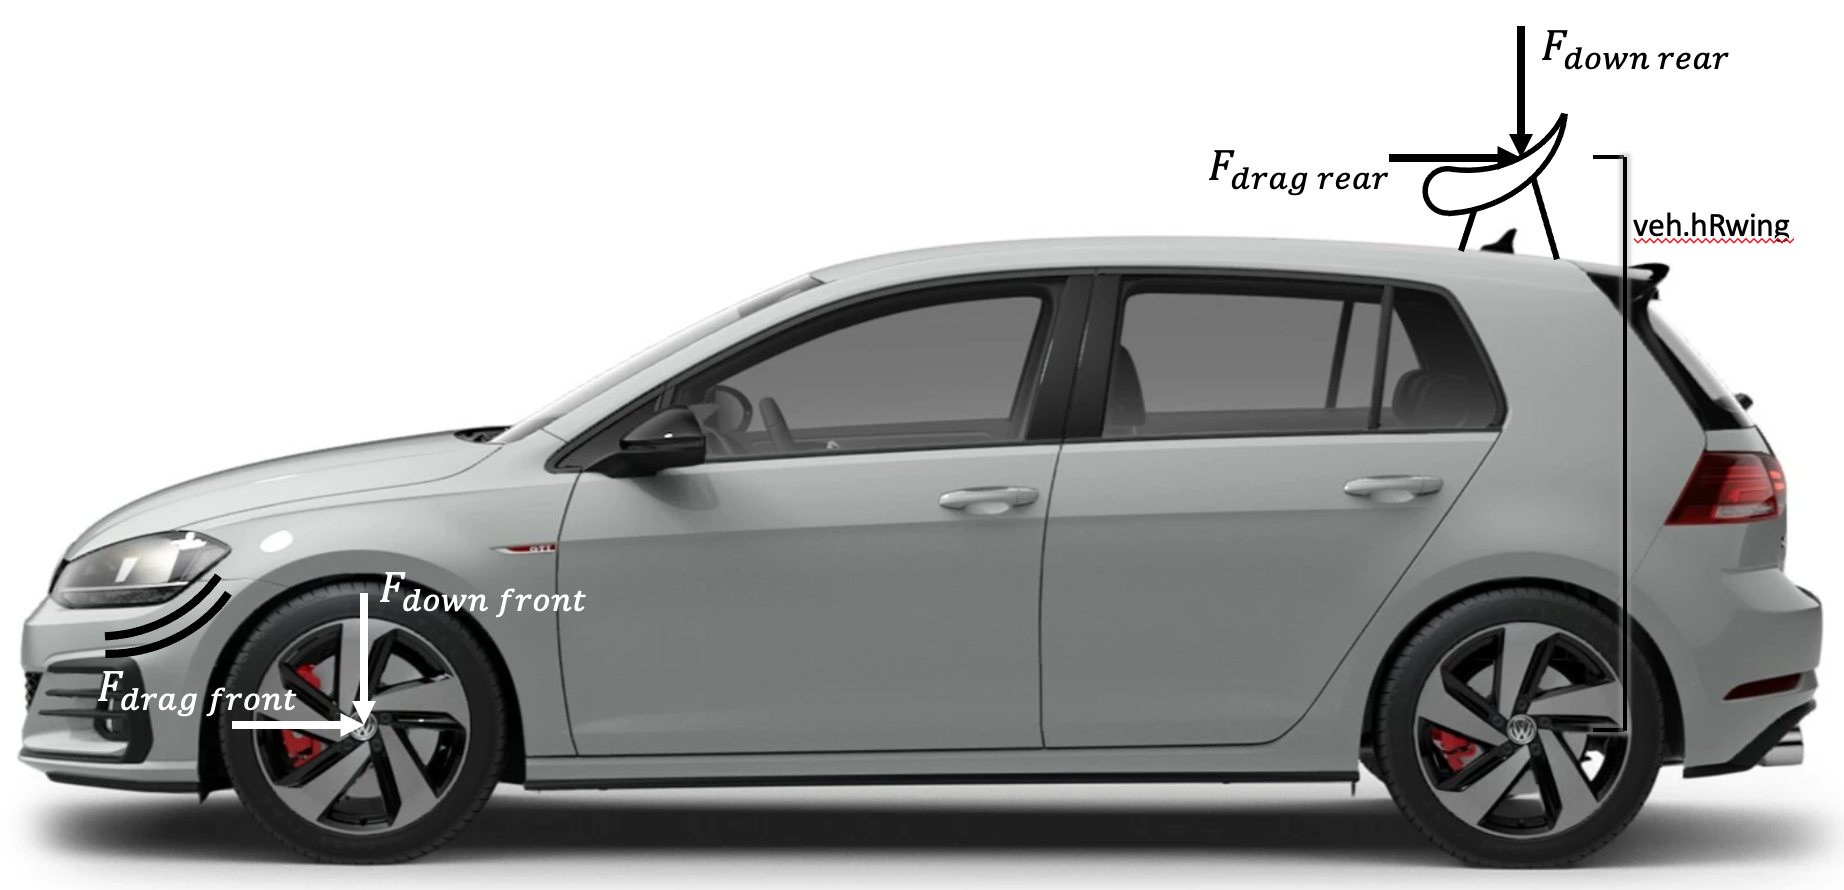
\includegraphics[width=400pt]{Template/Problem4/fbd_gti.png}
\url{https://www.vw.com/en/models/golf-gti.html}
\end{center}

\textit{Note: The drag on the rear wing will have an impact on the downforce on the front axle. Be sure to account for this.}

Restore Niki's brake distribution to the original 64/36.  Now, simulate the same curve as in the previous problem.   How does the distance covered compare to Question 3C?  How does the maximum lateral error compare to 3C? Plot the front and rear tire forces. Provide the plots and describe what is happening.  Does it make sense to add an aero kit to Niki?

\vspace*{0.5cm}

\expect{Run the simulation and answer the questions about the vehicle's behavior.  Was it a good idea to upgrade Niki? Include the tire force plots.}

\iftoggle{condensed}{
    \vspace*{0.5cm}
}{
    \subsubsection*{Solution:}
}

\iftoggle{solution}{
    %---------------------------------------------------------------------------------
% QUESTION 4.A
%---------------------------------------------------------------------------------
\secMOGS{Adding Aerodynamics}

Modify \verb!aero_effects.m! to implement the added downforce and drag from the wing.  We can assume that the front wing aero forces act at the center of the front wheel and that the rear wing aero forces act at a distance \verb!veh.hRwing! directly above the rear wheel. We can also assume that the front wing acts equally on the left and right front wheels and that the rear wing acts equally on the left and right rear wheels. Here is a free body diagram of the GTI with the forces we added with the two wings.    

\begin{center}
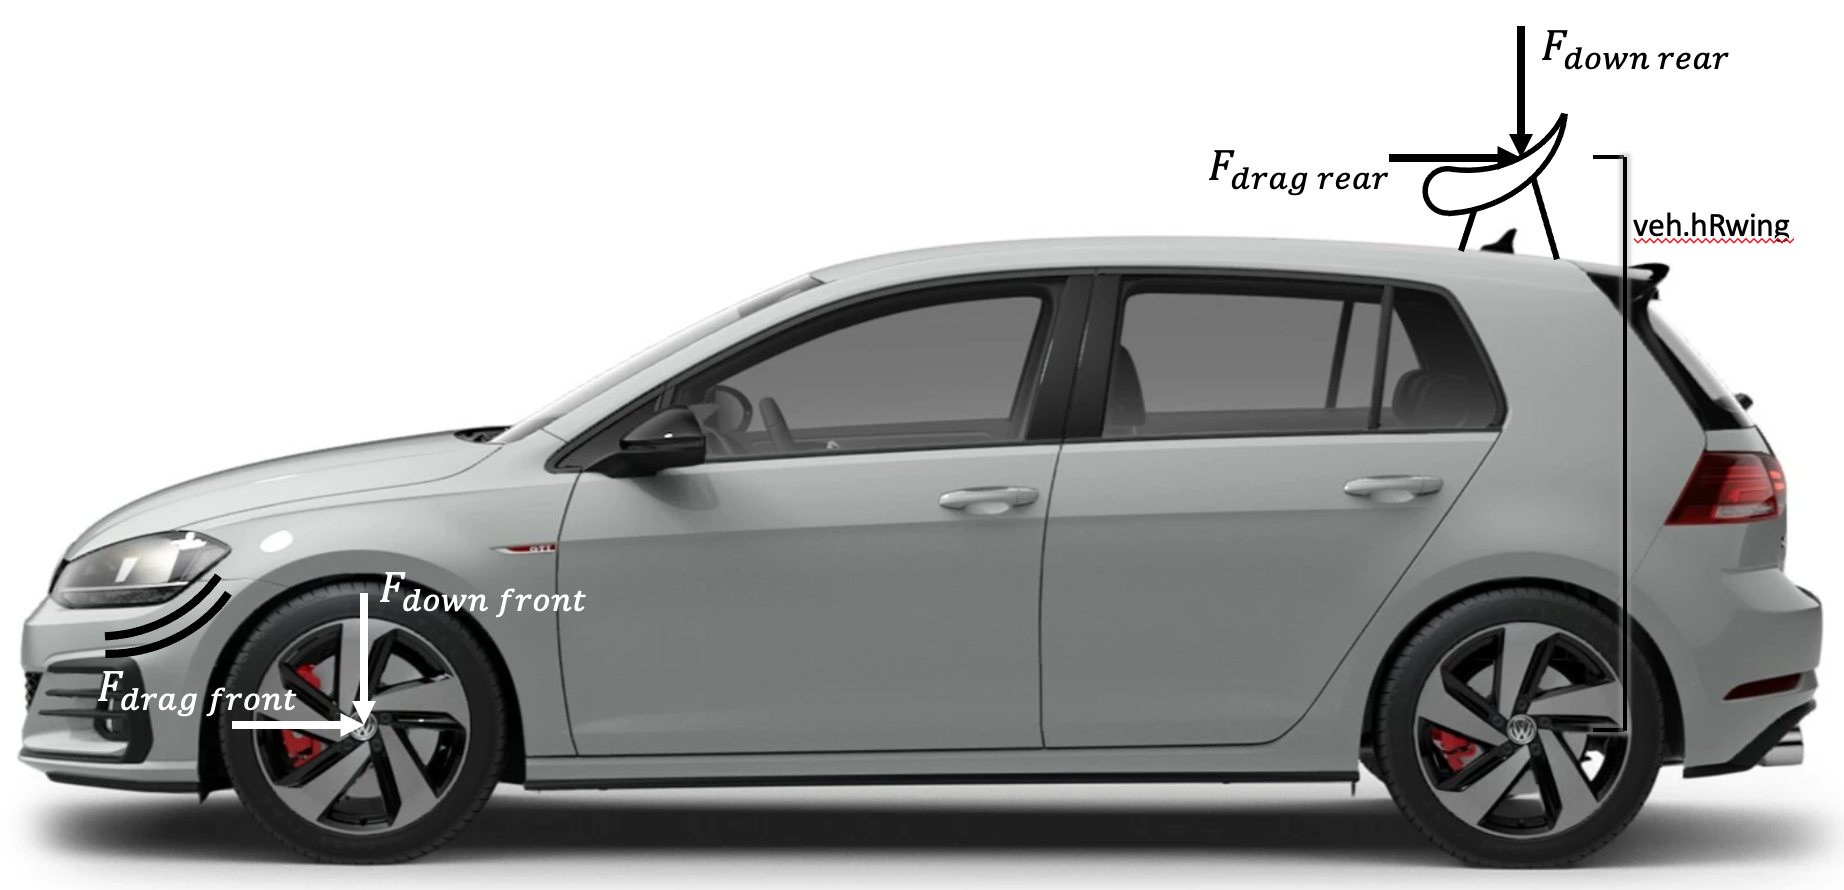
\includegraphics[width=400pt]{Template/Problem4/fbd_gti.png}
\url{https://www.vw.com/en/models/golf-gti.html}
\end{center}

\textit{Note: The drag on the rear wing will have an impact on the downforce on the front axle. Be sure to account for this.}

Restore Niki's brake distribution to the original 64/36.  Now, simulate the same curve as in the previous problem.   How does the distance covered compare to Question 3C?  How does the maximum lateral error compare to 3C? Plot the front and rear tire forces. Provide the plots and describe what is happening.  Does it make sense to add an aero kit to Niki?

\vspace*{0.5cm}

\expect{Run the simulation and answer the questions about the vehicle's behavior.  Was it a good idea to upgrade Niki? Include the tire force plots.}

\iftoggle{condensed}{
    \vspace*{0.5cm}
}{
    \subsubsection*{Solution:}
}

\iftoggle{solution}{
    %---------------------------------------------------------------------------------
% QUESTION 4.A
%---------------------------------------------------------------------------------
\secMOGS{Adding Aerodynamics}

Modify \verb!aero_effects.m! to implement the added downforce and drag from the wing.  We can assume that the front wing aero forces act at the center of the front wheel and that the rear wing aero forces act at a distance \verb!veh.hRwing! directly above the rear wheel. We can also assume that the front wing acts equally on the left and right front wheels and that the rear wing acts equally on the left and right rear wheels. Here is a free body diagram of the GTI with the forces we added with the two wings.    

\begin{center}
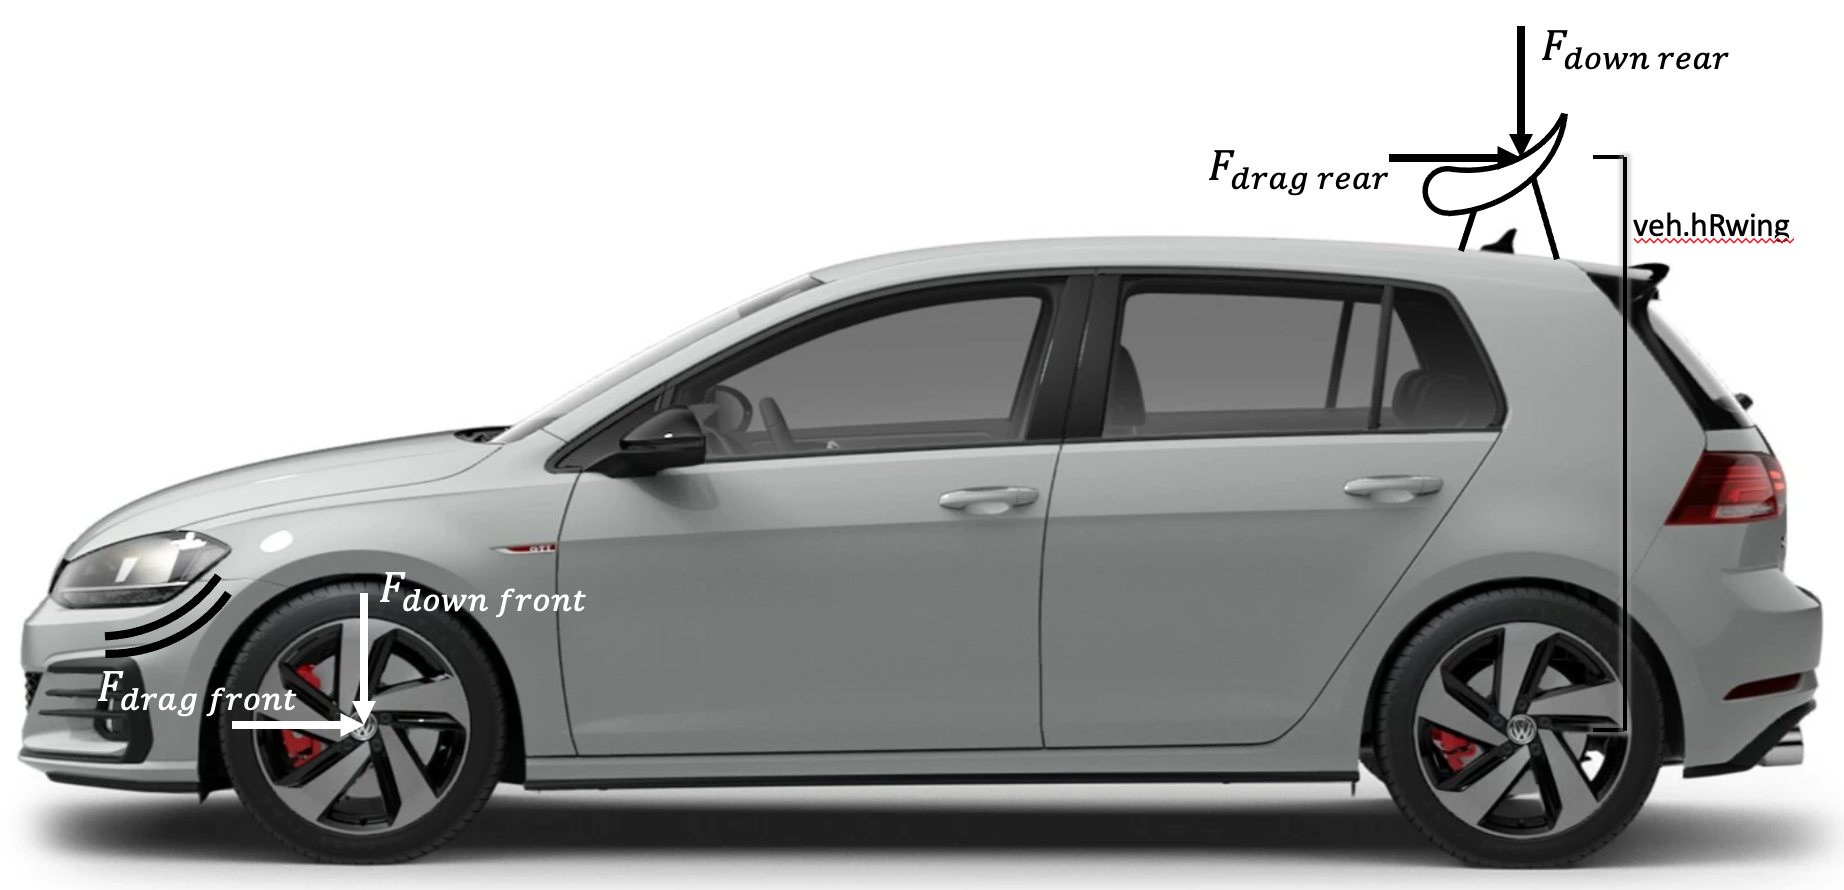
\includegraphics[width=400pt]{Template/Problem4/fbd_gti.png}
\url{https://www.vw.com/en/models/golf-gti.html}
\end{center}

\textit{Note: The drag on the rear wing will have an impact on the downforce on the front axle. Be sure to account for this.}

Restore Niki's brake distribution to the original 64/36.  Now, simulate the same curve as in the previous problem.   How does the distance covered compare to Question 3C?  How does the maximum lateral error compare to 3C? Plot the front and rear tire forces. Provide the plots and describe what is happening.  Does it make sense to add an aero kit to Niki?

\vspace*{0.5cm}

\expect{Run the simulation and answer the questions about the vehicle's behavior.  Was it a good idea to upgrade Niki? Include the tire force plots.}

\iftoggle{condensed}{
    \vspace*{0.5cm}
}{
    \subsubsection*{Solution:}
}

\iftoggle{solution}{
    %---------------------------------------------------------------------------------
% QUESTION 4.A
%---------------------------------------------------------------------------------
\secMOGS{Adding Aerodynamics}

Modify \verb!aero_effects.m! to implement the added downforce and drag from the wing.  We can assume that the front wing aero forces act at the center of the front wheel and that the rear wing aero forces act at a distance \verb!veh.hRwing! directly above the rear wheel. We can also assume that the front wing acts equally on the left and right front wheels and that the rear wing acts equally on the left and right rear wheels. Here is a free body diagram of the GTI with the forces we added with the two wings.    

\begin{center}
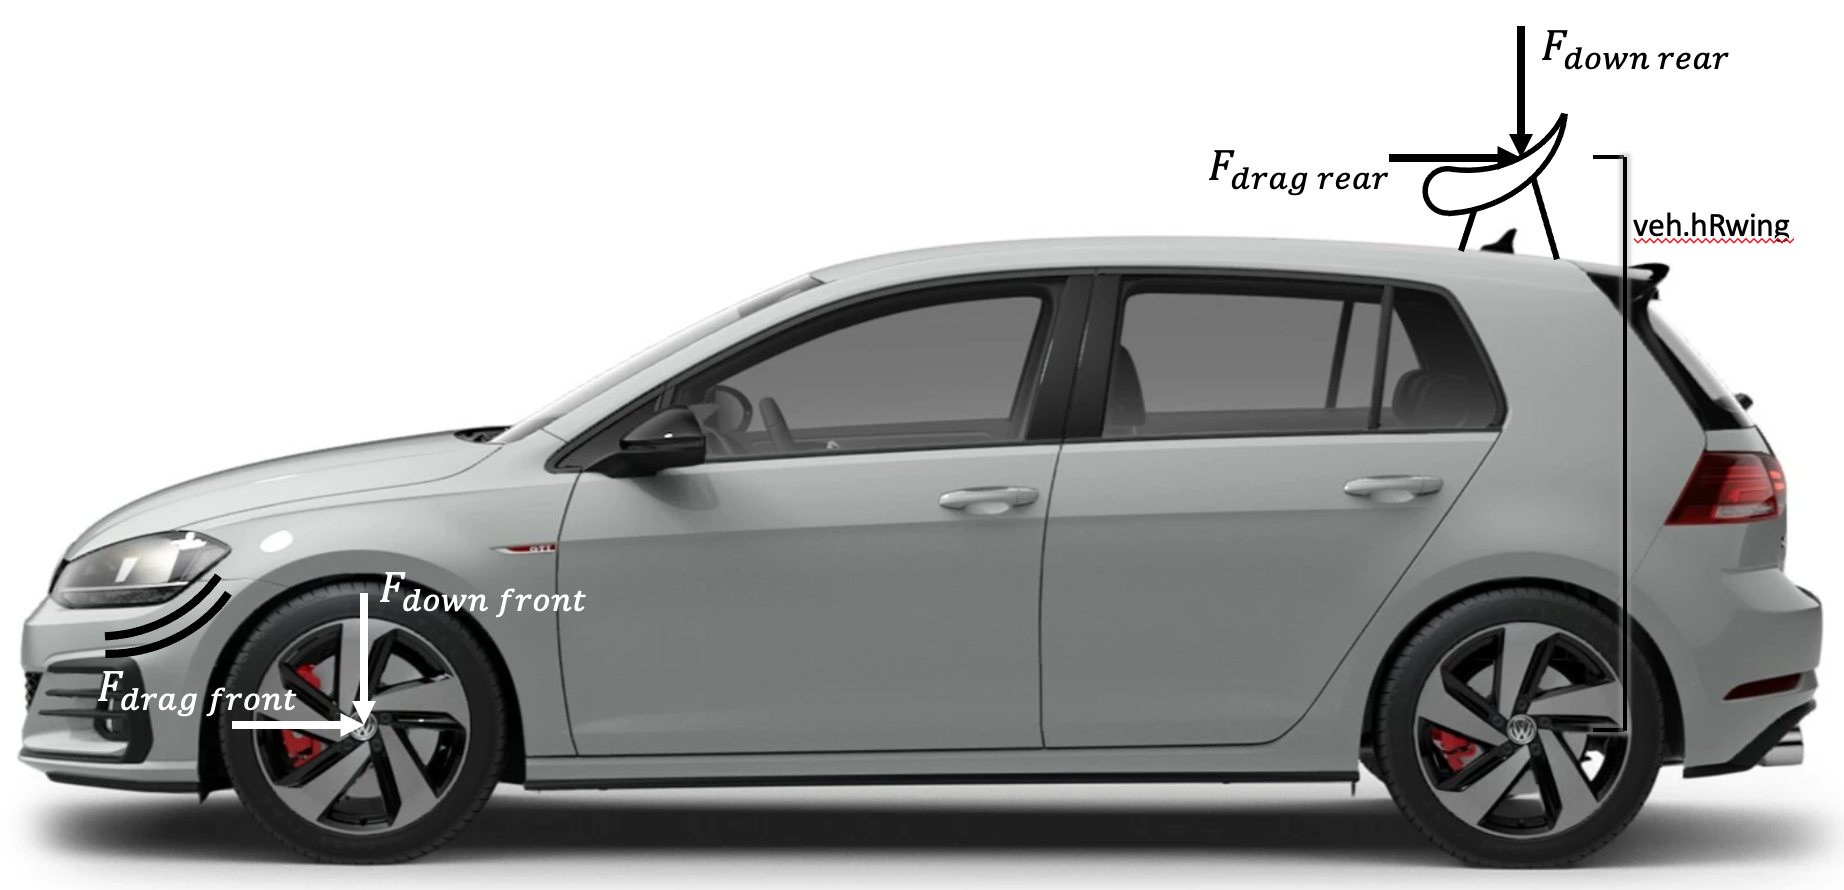
\includegraphics[width=400pt]{Template/Problem4/fbd_gti.png}
\url{https://www.vw.com/en/models/golf-gti.html}
\end{center}

\textit{Note: The drag on the rear wing will have an impact on the downforce on the front axle. Be sure to account for this.}

Restore Niki's brake distribution to the original 64/36.  Now, simulate the same curve as in the previous problem.   How does the distance covered compare to Question 3C?  How does the maximum lateral error compare to 3C? Plot the front and rear tire forces. Provide the plots and describe what is happening.  Does it make sense to add an aero kit to Niki?

\vspace*{0.5cm}

\expect{Run the simulation and answer the questions about the vehicle's behavior.  Was it a good idea to upgrade Niki? Include the tire force plots.}

\iftoggle{condensed}{
    \vspace*{0.5cm}
}{
    \subsubsection*{Solution:}
}

\iftoggle{solution}{
    \input{Solutions/Problem4/problem4a.tex}
    \newpage
}

\iftoggle{template}{
    \begin{solutionorbox}[3.5in]
    \end{solutionorbox}
    \newpage
}

\iftoggle{student}{
%---------------------------------------------------------------------------------
% STUDENT: BEGIN WORK
%---------------------------------------------------------------------------------


% Please box final answer

%---------------------------------------------------------------------------------
% STUDENT: END WORK
%---------------------------------------------------------------------------------
    \newpage
}












    \newpage
}

\iftoggle{template}{
    \begin{solutionorbox}[3.5in]
    \end{solutionorbox}
    \newpage
}

\iftoggle{student}{
%---------------------------------------------------------------------------------
% STUDENT: BEGIN WORK
%---------------------------------------------------------------------------------


% Please box final answer

%---------------------------------------------------------------------------------
% STUDENT: END WORK
%---------------------------------------------------------------------------------
    \newpage
}












    \newpage
}

\iftoggle{template}{
    \begin{solutionorbox}[3.5in]
    \end{solutionorbox}
    \newpage
}

\iftoggle{student}{
%---------------------------------------------------------------------------------
% STUDENT: BEGIN WORK
%---------------------------------------------------------------------------------


% Please box final answer

%---------------------------------------------------------------------------------
% STUDENT: END WORK
%---------------------------------------------------------------------------------
    \newpage
}












    \newpage
}

\iftoggle{template}{
    \begin{solutionorbox}[3.5in]
    \end{solutionorbox}
    \newpage
}

\iftoggle{student}{
%---------------------------------------------------------------------------------
% STUDENT: BEGIN WORK
%---------------------------------------------------------------------------------


% Please box final answer

%---------------------------------------------------------------------------------
% STUDENT: END WORK
%---------------------------------------------------------------------------------
    \newpage
}











